\subsection{Motivation}
\label{sec:fake.mct}
The processes leading to FNP leptons depend on the selection applied in the analysis. For instance, a selection with same-sign leptons 
will have contributions from top quark pair production (\ttbar) or the associated production of a vector boson and jets 
($W$+jets or $Z$+jets).%, or opposite sign $W$ pair production ($W^+W^-$). 
These processes cannot give two leptons of the same electric charge unless there is a charge mis-measurement (mainly affecting electrons) 
or that a FNP lepton was produced. It is possible to generate the processes that can contribute to a FNP lepton, such as \ttbar or 
$V$+jets, with Monte Carlo event generators processed through Geant4 detector simulation of the ATLAS detector.  
This approach will yield an estimate however it might not be reliable. For instance, the detector simulation itself might not 
reproduce the true behavior of the interaction of the physics objects with the detector, particularly when looking at rare processes 
such as the production of FNP leptons. The second limitation is in the generation of enough MC events to probe the region of the 
phase space targeted by the analysis which affects the statistical uncertainties in the estimates.
The latter concern is addressed by ensuring that the simulations for the major backgrounds (\ttbar and $V$+jets) have much 
higher event count than the corresponding number of events observed in the data sample.
In fact, these backgrounds have a large number of simulated events because they are important for many analyses 
(including SM measurements and BSM searches).
The rest of the section will concentrate on addressing the former limitation. 

%% ****
%% low statistics of the tri-lepton samples and the variety of sources of fake leptons.
%% It is difficult to rely on data-driven (including ME-based) methods that rely on inverting the isolation requirement given we deal with multi-jet final states. Inversion of the isolation requirement produces a sample with much more energetic jets than in the sample with the un-inverted isolation. 

%% ''
%% picked variables that offer good separation between processed with prompt and ``fake'' leptons.
%% It is nice that the corrections are close to one but they do not have to be. For example, their deviations from unity depend on the decay modes of heavy flavor hadrons that are implemented in simulations.

%% Is the showering of the samples used to measure the correction of the fake rate and the that of the samples it is applied to the same? if not, is there a potential systematic difference that has to be taken into account?

%% We used Herwig for showering of all the samples that require corrections to the fake rates.



\subsection{Description of the method}

The MC template method relies on the correct modelling of FNP leptons kinematics in 
MC simulation to extrapolate background predictions from control regions to the signal regions.
The method assumes that the kinematic shapes for each source of FNP lepton is correctly modeled in the simulations, 
and the normalization for each source is extracted in a combined fit to data control regions.
The number of normalization factors depend on the number of identified origins of the FNP lepton in the signal regions
and the control regions are designed to constrain these factors in regions enriched with FNP leptons from the same origin.

To illustrate the approach, we describe the application of the method in SS/3L analysis later described in this thesis.
The processes of interest that may lead to a FNP lepton or a charge flip are $\ttbar$ and $V$+jets. 
FNP leptons are classified using an algorithm that navigates the generator particle record to determine where the FNP lepton 
is originating from. 
The lepton is classified as either an electron or a muon that is prompt from decays of on-shell $W$ and $Z$ bosons, 
non-prompt from a heavy flavor $b$ decay (HF), or fake from mis-identification of a light flavor jet or a photon (LF). 
In the case of an electron, we further classify the prompt electrons to prompt electrons with the correct charge or with a 
charge mis-measurement, commonly named charge flip.
In total, five categories referred to as MC templates are construed following the classification illustrated 
in figure~\ref{Fig:fakes_classification}.

\begin{figure}[t!]
\centering
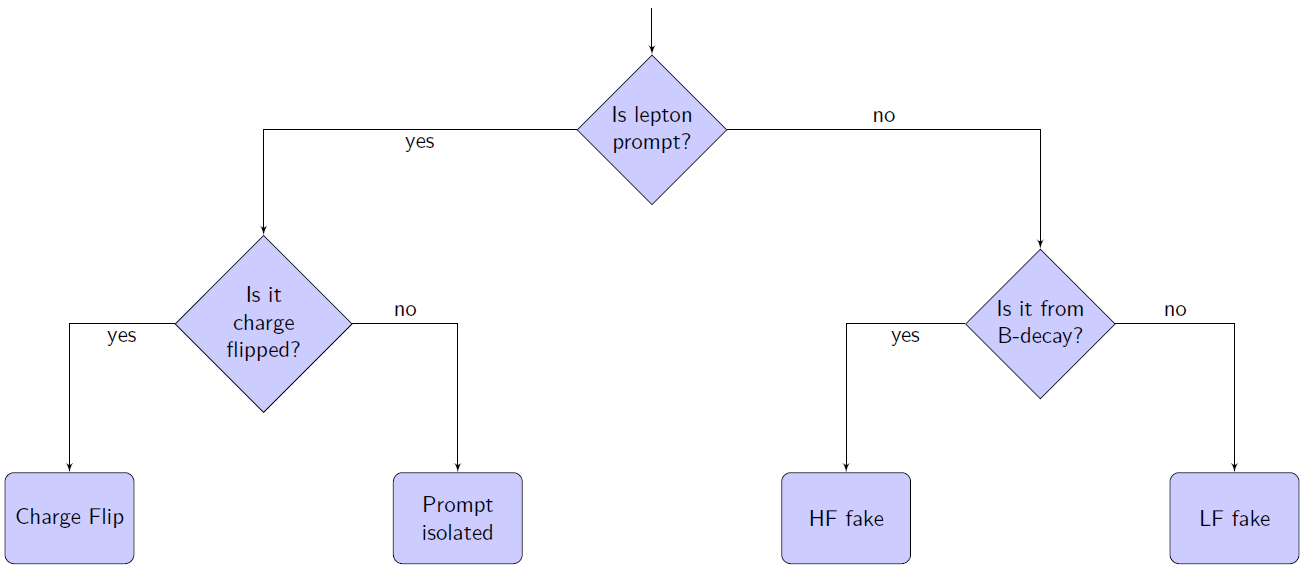
\includegraphics[width=0.7\textwidth]{mct/MC-tmpl}
\caption
{Lepton classification.
}
\label{Fig:fakes_classification}
\end{figure}

\subsection{Correction factors}

The FNP estimate relies on kinematic extrapolation using processes expected to contribute via FNP leptons from control regions 
with low jet multiplicity and \met, to the signal regions that require high jet multiplicity and \met. 
The control regions are chosen to separate FNP leptons from HF origins and FNP leptons from LF origins.
For instance, a control sample characterized by the presence of a $b$-jet will be enriched in processes with one FNP lepton that is 
coming from a HF decay, while a sample characterized by the absence of a $b$-jet will have one FNP lepton from LF decay.
The presence of one FNP lepton in the control sample allows the correction of the production rate of these FNP leptons 
by performing a fit to data. 

For example, if a Z$\to\mu\mu$+LF jet event is reconstructed as a $\mu^+\mu^-e^+$ event, then the electron is fake.
Therefore, a correction of LF jet $\to$ e (Fr(LF$\to$e)) is applied to the rate of $\mu\mu e$ events. The correction Fr(LF$\to$e)
is constrained by a fit to data in control regions dominated by LF jet $\to$ e type fakes. 
Similarly, three other corrections are defined as LF jet $\to\mu$ (Fr(LF$\to\mu$)),  HF jet $\to$ e (Fr(HF$\to$e)),  
HF jet $\to\mu$ (Fr(HF$\to\mu$)). An additional correction is applied to correct the charge flip rate predicted by simulation.
For example, a Z$\to e^+e^-$ event is reconstructed as $e^+e^+$ or $e^-e^-$. The simulation takes into account the charge flip 
rate but it might be off. The charge flip (Cf(e)) correction derived from a data fit is expected to recover this mis-modeling.
The charge flip rate only concern electrons as the muon charge flip rate is negligible.

A likelihood fit is defined as the product of the Poisson probabilities describing the observed events in the binned 
distributions from the expected number of events rescaled by the five multipliers which are left free to float in the fit.  
These multipliers are applied to the MC predictions in the signal regions to obtain an estimation of the charge flip and FNP backgrounds.

\subsection{Control regions}

The corrections depend on the simulated sample,
the reconstructed final state, and the flavor of the leptons. As a result, care must be taken when designing the control regions 
used to perform the fit of the FNP leptons and electron charge flip templates. 
For instance, each template needs to be constrained in a selection that is representative of the processes leading to 
FNP leptons and charge flip electrons present in the kinematic region targeted by the search for BSM physics. 

In the SS/3L analysis discussed in this thesis the control regions are defined with at least two same-sign 
leptons, $\met>40$~GeV, two or more jets. This pre-selection ensures that the FNP leptons are not from fakes originating from 
QCD like event topologies. 
They are further split in regions 
with or without $b$-jets to constrain the HF and LF leptons respectively. In addition, they are also split with different 
flavours of the same-sign lepton pair ee, e$\mu$, and $\mu\mu$, giving a total of six control regions. 
Any event entering the signal region is vetoed. The ee channel will constrain the charge flip correction factor, fake leptons 
 from LF decays in the selection without $b$-jets, and non-prompt decay from HF in the selection with $b$-jets. 
The $\mu\mu$ channel will constrain the muon fake rates in the LF and HF decays for the selection without or with $b$-jets, 
respectively. The e$\mu$ channel will constrain both the electron and muon fakes for events containing both lepton flavors. 

The six distributions are chosen for variables that provide the best separation between processes with prompt leptons and processes with FNP leptons and charge flip and are shown 
before and after the fit in Figures \ref{f:prefit_CR0b}-\ref{f:prefit_CR1b} and Figures \ref{f:postfit_CR0b}-\ref{f:postfit_CR1b}, respectively. 

 \begin{figure}[!htb]
   \includegraphics[width=.32\textwidth]{mct/Prefit/el2_pt_ee_CR0b_SS3L}
   \includegraphics[width=.32\textwidth]{mct/Prefit/NJETS_em_CR0b_SS3L}
   \includegraphics[width=.32\textwidth]{mct/Prefit/mu2_pt_mm_CR0b_SS3L}
 \caption{
 Pre-fit distributions for  $ee$ channel (left),  for  $e\mu$ channel (middle), and  for  $\mu\mu$ channel (right) from CR0b that were used in the fit to extract the FNP lepton and charge flip multipliers.
The generator used in these plots is Powheg. The hashed band represents the sum of systematic uncertainties on the predictions.
 \label{f:prefit_CR0b}
 }
 \end{figure}

\begin{figure}[!htb]
  \includegraphics[width=.32\textwidth]{mct/Postfit/el2_pt_ee_CR0b_SS3L}
  \includegraphics[width=.32\textwidth]{mct/Postfit/NJETS_em_CR0b_SS3L}
  \includegraphics[width=.32\textwidth]{mct/Postfit/mu2_pt_mm_CR0b_SS3L}
\caption{
Post-fit distributions for  $ee$ channel (left),  for  $e\mu$ channel (middle), and  for  $\mu\mu$ channel (right) from CR0b that were used in the fit to extract the FNP lepton and charge flip multipliers.
The generator used in these plots is Powheg. The hashed band represents the sum of systematic uncertainties on the predictions.
\label{f:postfit_CR0b}
}
\end{figure}

 \begin{figure}[!htb]
   \includegraphics[width=.32\textwidth]{mct/Prefit/el2_pt_ee_CR1b_SS3L}
   \includegraphics[width=.32\textwidth]{mct/Prefit/NJETS_em_CR1b_SS3L}
   \includegraphics[width=.32\textwidth]{mct/Prefit/mu2_pt_mm_CR1b_SS3L}
 \caption{
 Pre-fit distributions for  $ee$ channel (left), for  $e\mu$ channel (middle), and  for  $\mu\mu$ channel (right) from CR1b that were used in the fit to extract the FNP lepton and charge flip multipliers.
The generator used in these plots is Powheg. The hashed band represents the sum of systematic uncertainties on the predictions.
 \label{f:prefit_CR1b}
 }
 \end{figure}

\begin{figure}[!htb]
  \includegraphics[width=.32\textwidth]{mct/Postfit/el2_pt_ee_CR1b_SS3L}
  \includegraphics[width=.32\textwidth]{mct/Postfit/NJETS_em_CR1b_SS3L}
  \includegraphics[width=.32\textwidth]{mct/Postfit/mu2_pt_mm_CR1b_SS3L}
\caption{
Post-fit distributions for  $ee$ channel (left), for  $e\mu$ channel (middle), and  for  $\mu\mu$ channel (right) from CR1b that were used in the fit to extract the FNP lepton and charge flip multipliers.
The generator used in these plots is Powheg. The hashed band represents the sum of systematic uncertainties on the predictions.
\label{f:postfit_CR1b}
}
\end{figure}

The minimization of the negative log likelihood using the \textsc{Minuit} package leads 
to the multipliers shown in Tables \ref{t:fake_factors_powheg} and \ref{t:fake_factors_sherpa}.
The tables represent the multipliers obtained from the fit upon using two different parton showers, \POWHEGBOX and \SHERPA 
for the processes that lead to FNP leptons and charge flips.
The systematic uncertainty is obtained by varying the 
generator from \POWHEGBOX to \SHERPA and evaluating the impact on the expected background from FNP and charge flip leptons. 
It is found to be the dominant contribution to the systematic uncertainty of the method (up to 80\%).
The uncertainties in the multipliers themselves correspond to how much the parameter needs to be varied for 
a one standard deviation change in the likelihood function. This uncertainty takes into account the limited number of simulated events and is included as a 
systematic uncertainty on the expected number of background events. 

\begin{table}[!htb]
  \caption{The FNP and charge flip multipliers obtained after minimizing the likelihood function using Pythia.
    The uncertainty in the multipliers takes into account the limited statistics of simulated events.
    \label{t:fake_factors_powheg}}
  \centering
  % % \scalebox{0.85}{
   \begin{tabular}{|c|c|c|}
          \hline
          Category & Multiplier & Uncertainty  \\
          \hline
          chFlip & 1.49 & 0.58 \\ 
          HF EL & 2.80 & 0.98 \\
          LF EL & 2.89 & 0.88 \\
          HF MU & 1.59 & 0.31 \\
          LF MU & 1.00 & 1.34 \\
          \hline
        \end{tabular}
  % % }                                                                            
\end{table}

\begin{table}[!htb]
  \caption{The FNP and charge flip multipliers obtained after minimizing the likelihood function using Sherpa.
    The uncertainty in the multipliers takes into account the limited statistics of simulated events.
    \label{t:fake_factors_sherpa}}
  \centering
  % % \scalebox{0.85}{
  \begin{tabular}{|c|c|c|}
    \hline
    Category & Multiplier & Uncertainty  \\
    \hline
    chFlip & 1.34 & 0.58 \\ 
    HF EL & 2.40 & 0.85 \\
    LF EL & 1.83 & 1.04 \\
    HF MU & 1.17 & 0.16 \\
    LF MU & 2.40 & 0.81 \\
    \hline
  \end{tabular}                                                                                         
  % % }                                                                            
\end{table}
